\documentclass[conference]{IEEEtran}
\IEEEoverridecommandlockouts
\usepackage{hyperref}       % hyperlinks
\usepackage{url}            % simple URL typesetting
\usepackage{booktabs}       % professional-quality tabless
\usepackage{amsfonts}       % blackboard math symbols
\usepackage{amsmath}
\usepackage{nicefrac}       % compact symbols for 1/2, etc.
\usepackage{microtype}      % microtypography
\usepackage{cleveref}       % smart cross-referencing
\usepackage{graphicx}
\usepackage[english]{babel}
\usepackage{csquotes}
\usepackage{multirow}

% Bibliography
\usepackage[%
    backend=biber,%
    backref=false,%
    giveninits=true,%
    autocite=inline,%
    sorting=none,%
    sortcites=true,%
    mincitenames=1,%
    maxcitenames=2,%
    maxbibnames=10,%
    doi=true,%
    isbn=false,%
    url=false,%
    natbib=false,
]{biblatex}

\renewcommand*{\bibfont}{\small}

\addbibresource{../discography.bib}


\begin{document}

\title{Training Dense Object Nets: A Novel Approach}

\author{\IEEEauthorblockN{1\textsuperscript{st} Kanishk Navale}
    \IEEEauthorblockA{\textit{Sereact GmbH.} \\
        \textit{}
        Stuttgart, Germany \\
        kanishk.navale@sereact.ai}
    \and
    \IEEEauthorblockN{2\textsuperscript{nd} Ralf Gulde}
    \IEEEauthorblockA{\textit{Sereact GmbH.} \\
        \textit{}
        Stuttgart, Germany \\
        ralf.gulde@sereact.ai}
    \and
    \IEEEauthorblockN{3\textsuperscript{rd} Marc Tuscher}
    \IEEEauthorblockA{\textit{Sereact GmbH.} \\
        \textit{}
        Stuttgart, Germany \\
        marc.tuscher@sereact.ai}
    \and
    \IEEEauthorblockN{4\textsuperscript{th} Oliver Riedel}
    \IEEEauthorblockA{\textit{ISW - Universität Stuttgart} \\
        \textit{}
        Stuttgart, Germany \\
        oliver.riedel@isw.uni-stuttgart.de}
}

\maketitle

\begin{abstract}
    Our work proposes a novel framework that addresses the computational limitations associated with training Dense Object Nets (DON)
    while achieving robust and dense visual object descriptors. DON's descriptors are known for their robustness to
    viewpoint and configuration changes, but training these requires image pairs with computationally expensive correspondence mapping.
    This limitation hampers dimensionality and robustness, thereby restricting object generalization.
    To overcome this, we introduce data generation procedure using synthetic augmentation and a novel deep learning architecture
    that produces denser visual descriptors with reduced computational demands. Notably, our framework eliminates the need for
    image pair correspondence mapping and showcases its application in a robotic grasping pipeline.
    Experimental results demonstrate that our approach yields descriptors as robust as those generated by DON.
\end{abstract}

\begin{IEEEkeywords}
    Dense Object Nets, robot grasping, generalized object representation, reduced computation costs.
\end{IEEEkeywords}

\section{Introduction}
The objectives of long-standing robotics and robotic manipulation are to create a general-purpose robot capable of carrying out practical activities like Chappie~\cite{blomkamp2015chappie} or C-3PO~\cite{lucas1977star}. While advancements have been made recently in adjacent domains, achieving this goal remains a work in progress. For instance, AlphaGo~\cite{silver2018general},
a game-playing artificial intelligence system trained entirely on self-play, defeated the world's best human Go player at the time. Subsequently, \citeauthor{silver2016mastering}~\cite{silver2016mastering}
developed artificial intelligence algorithms that mastered the game of chess, Go, World of Warcraft~\cite{entertainment2013world}, and Shogi,
surpassing human playing expertise. Most of these algorithms learn directly from visual data, such as gameplay recordings or online video streams, emphasizing the importance of visual data in AI. Meanwhile, the launch of AlexNet~\cite{krizhevsky2017imagenet} in 2012 transformed the field of computer vision. Other visual tasks, such as semantic segmentation~\cite{long2015fully}, object identification and recognition~\cite{he2017mask}, and human pose estimation~\cite{guler2018densepose}, have also witnessed significant gains in recent years. Significant breakthroughs have been made in robotics, ranging from self-driving cars to humanoid robots capable of performing complex tasks using cameras and other vision sensors. Despite these advancements, the most frequently used robotic manipulation systems have evolved slightly in the previous 30 years. Typical auto-factory robots continue to perform repetitive operations such as welding and painting, following a pre-programmed course with no feedback from the surroundings. If we want to increase the utility of our robots, we must move away from highly controlled settings and robots that perform repetitive actions with little feedback or adaptability capabilities. Liberating ourselves from these constraints of controlled settings-based manufacturing would allow us to enter new markets, as witnessed by the proliferation of firms~\cite{sereact} competing in the logistics domain.

The ideal object representation for robot grasping and manipulation tasks remains to be engineered today.
Existing representations may not be suitable for complex tasks due to limited capabilities of understanding an object's geometrical and structural information.
In \citeyear{florence2018dense}, \citeauthor{florence2018dense}~\cite{florence2018dense} introduced a novel visual
object representation to the robotics community,  terming it ``dense visual object descriptors''. DON, an artificial intelligence
framework proposed by
\Citeauthor{florence2018dense}~\cite{florence2018dense} produces dense visual object descriptors. In detail, the DON converts every pixel in the
image ($I[u, v] \in \mathbb{R}^3$) to a higher dimensional embedding ($I_D[u, v] \in \mathbb{R}^D$) such that $D \in \mathbb{N}^+$ consuming
image-pair correspondences as input yielding pixelwise embeddings
which are nothing but dense local descriptors.
The dense visual object descriptor generalizes an object up to a certain extent and has been recently
applied to rope manipulation \cite{rope-manipulation},
block manipulation \cite{block-manipulation}, robot control \cite{florence2019self}, fabric manipulation \cite{fabric-manipulation} and
robot grasp pose estimation \parencites{kupcsik2021supervised}{adrian2022efficient}. \citeauthor{adrian2022efficient}~\cite{adrian2022efficient}
further demonstrated that DON can be trained on synthetic data and still generalize to real-world objects. Furthermore, \citeauthor{adrian2022efficient}~\cite{adrian2022efficient} demonstrated that
the quality of descriptors produced by the DON framework depends on the higher or longer embedding dimension. We tried training the DON on a computation
device equipped with NVIDIA RTX A6000 GPU with 48GB VRAM. However, we could not train the DON to produce a higher embedding dimension due to the limited VRAM.
The DON framework is computationally expensive, as shown in Table~\ref{table:don_gpu_bechmark}, and limits the user to generalize objects to a certain extent making it
difficult to use as a robot grasping pipeline in real-world logistics and warehouse automation scenarios.

\begin{table}[htb]
    \caption{Benchmark of DON framework trained on GPU with 48GB VRAM with 128 image-pair correspondences, batch size of 1 and ``Pixelwise NTXENT Loss''~\cite{adrian2022efficient} as a loss function.}
    \label{table:don_gpu_bechmark}
    \centering
    \begin{tabular}{lllll}
        \toprule
        \multicolumn{5}{c}{GPU VRAM consumption to train DON}   \\
        \midrule
        Descriptor Dimension & 3     & 8      & 16     & 32     \\
        VRAM Usage (GB)      & 9.377 & 13.717 & 20.479 & 30.067 \\
        \bottomrule
    \end{tabular}
\end{table}

To overcome the computation resource limitation to produce denser visual object descriptors, we propose a novel framework to
train and extract dense visual object descriptors produced by DON, which is computationally efficient.

\section{Related Works}
We are solely interested in computing dense visual object descriptors of an object.
The DON training strategy in \cite{florence2018dense} relies on the depth information for computing correspondences in an image pair using
camera intrinsics and pose information \cite{hartley2003multiple}.
However, when employing consumer-grade depth cameras for capturing the depth information,
the depth cameras capture noisy depth in cases of tiny, reflecting objects, which are common in
industrial environments. In the meantime, \citeauthor{kupcsik2021supervised}~\cite{kupcsik2021supervised} used Laplacian Eigenmaps \cite{belkin2003laplacian}
to embed a 3D object model into an optimally generated embedding space acting as a target to train DON in a supervised fashion.
The optimal embeddings bring more domain knowledge by associating the 3D object model with image views.
\citeauthor{kupcsik2021supervised}~\cite{kupcsik2021supervised} efficiently apply it to smaller, texture-less and
reflective objects by eliminating the need for depth information. \citeauthor{kupcsik2021supervised}~\cite{kupcsik2021supervised}
further, compare training strategies for producing 6D grasps for industrial objects and show that a unique supervised training approach
increases pick-and-place resilience in industry-relevant tasks.

\citeauthor{florence2020dense}~\cite{florence2020dense} has found that the pixelwise contrastive loss function used to train DON might not perform well if a computed
correspondence is spatially inconsistent (analogously to the case of noisy depth information). Further highlighting that the precision
of contrastive-trained models can be sensitive to the
relative weighting between positive-negative sampled pixels. Instead, the \citeauthor{florence2020dense}~\cite{florence2020dense} introduces a new continuous
sampling-based loss function called ``Pixelwise Distribution Loss''.
The pixelwise distribution loss is much more effective as it is a smooth continuous pixel space sampling method compared to the
discrete pixel space sampling method based on pixelwise contrastive loss.
The pixelwise distribution loss regresses probability distribution heatmaps to minimize the divergence between the predicted
heatmap and the ground truth heatmap mitigating errors in correspondences. Furthermore, the pixelwise distribution loss does not
need non-matching correspondences compared to the
pixelwise contrastive loss.
Differently, \citeauthor{hadjivelichkov2021fully}~\cite{hadjivelichkov2021fully} extends the DON training using semantic correspondences between objects in multi-object
or cluttered scenes overcoming the limitations of \parencites{hartley2003multiple}{belkin2003laplacian}.
The authors, \citeauthor{hadjivelichkov2021fully}~\cite{hadjivelichkov2021fully} employ offline unsupervised clustering based on confidence in object similarities to generate hard and soft correspondence labels.
The computed hard and soft labels lead DON in learning class-aware dense object descriptors, introducing hard and soft margin constraints in the proposed pixelwise contrastive loss to train DON.
Further eliminating the need for camera pose and intrinsic information along with depth information to compute correspondences in an image pair, \citeauthor{nerf-Supervision}~\cite{nerf-Supervision} used
NeRF~\cite{mildenhall2021nerf} to train DON. The NeRF~\cite{mildenhall2021nerf} recreates a 3D scene from a sequence of images captured by the smartphone camera. The correspondences are extracted from
the synthetically reconstructed scene to train DON.
Recently, based on SIMCLR inspired frameworks~\parencites{chen2020simple}{zbontar2021barlow},
\citeauthor{adrian2022efficient}~\cite{adrian2022efficient} introduced similar architecture and another novel loss function called
Pixelwise NTXent loss to train DON more robustly.
The Pixelwise NTxent loss consumes synthetic correspondences independent of depth cameras computed from image augmentations to train DON.
\citeauthor{adrian2022efficient}'s experiments show that the novel loss function is invariant to the batch size.
Additionally adopted ``$PCK@k$''
metric has been adopted as in proceedings \parencites{chai2019multi}{fathy2018hierarchical} to evaluate and benchmark
DON on cluttered scenes previously not benchmarked.

In the proposed framework, we do not use any loss functions in
\parencites{florence2018dense}{florence2020dense}{kupcsik2021supervised}{adrian2022efficient}{hadjivelichkov2021fully}{nerf-Supervision} to train DON
however we adopt the network architecture from \cite{florence2018dense} and train on the task of the ``KeypointNet''\cite{suwajanakorn2018discovery}
with adaption of the loss functions proposed in \parencites{suwajanakorn2018discovery}{zhao2020learning}.

\section{Methodology}
In this section, we outline the methodologies employed.
Our approach encompasses synthetic dataset engineering,
a novel framework, loss function modifications and a comprehensive grasping pipeline.

Firstly, we focus on synthetic dataset engineering accommodating spatial, colour and background augmentation. The colour and
background augmentations help the framework to predict object-oriented descriptors.
Secondly, we present a novel framework designed to reduce computational resource consumption with loss function
modifications to optimize performance. Lastly, we introduce a comprehensive robot grasping pipeline exploiting the generalizing capabilities of our framework.

\subsection{Dataset Engineering}

We have chosen the cap object for creating a synthetic dataset as the cap mesh models are readily available in the Shapenet library~\cite{chang2015shapenet} as it contains rich object information, including textures.
Furthermore, we choose five cap models from the Shapenet library and use Blenderproc~\cite{blenderproc}
to generate the synthetic dataset. We save one RGB image, mask, and depth for each cap model from the synthetic scene.
Additionally, we employ synthetic augmentations as proposed in \cite{adrian2022efficient} to synthetically
spatial augment the cap's position and rotation in an image, including background randomization
using Torchvision~\cite{marcel2010torchvision} library. An augmented image pair is sampled randomly to generate camera poses for different viewpoints. Additionally, image-pair correspondences are computed
\footnote[1]{GitHub Link: \emph{link is made anonymous for the review}}
as illustrated in the Figure~\ref{fig:image_augs}. We only compute 24 image-pair correspondences
for an image-pair as we found that 24 image correspondences yield stable computation for translation and rotation for all the objects.
Using depth information,
we project the computed correspondences to the camera frame and compute the relative transformation between
two camera-frame coordinates of the correspondences using Kabsch's transformation~\cite{kabsch}.
Moreover, mask and depth images are not used during inference.

\begin{figure}[htb]
    \centering
    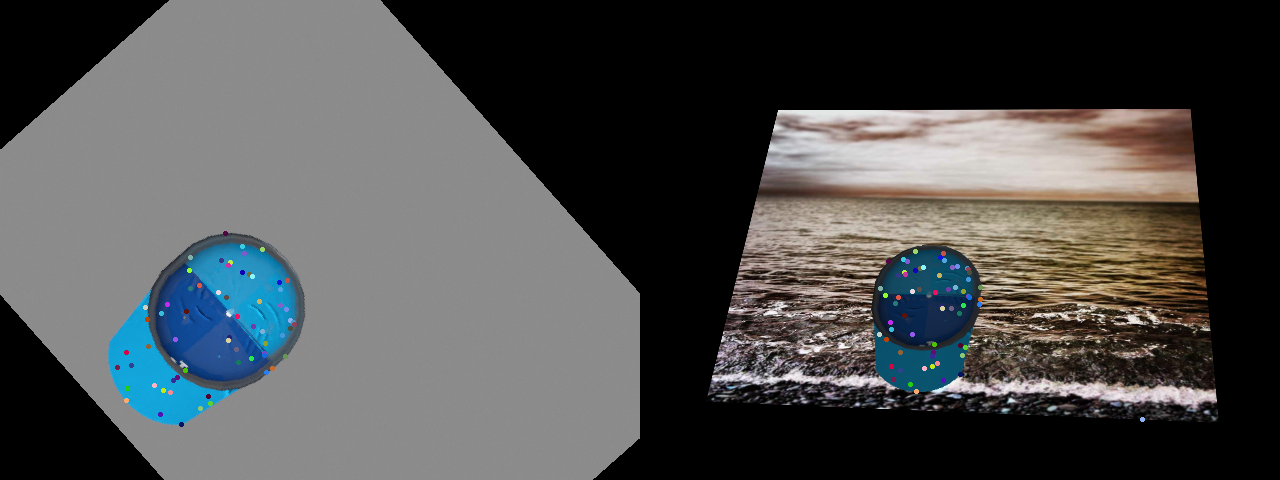
\includegraphics[scale=0.175]{images/debug_correspondences.png}
    \caption{Depiction of image synthetic spatial augmentation and correspondences mapping in an image-pair. The colored encoded dots in the figure represents correspondences in an image-pair.}
    \label{fig:image_augs}
\end{figure}


\subsection{Framework \& Mining Strategy}

As a backbone, we employ ResNet-34 architecture \cite{resnet}.
We preserve the last convolution layer and remove the pooling and linear layers. The backbone downsamples the RGB image $I_{RGB} \in \mathbb{R}^{H \times W \times 3}$
to dense features $I_d \in \mathbb{R}^{h \times w \times D}$
such that $ h \ll H, w \ll W \text{ and } D \in \mathbb{N}^+$.
We upsample the dense features from the identity layer
(being identical to the last convolution layer in the backbone) as illustrated in the Figure~\ref{fig:modified_dnn} in page~\pageref{fig:modified_dnn} as follows:
\begin{equation}
    f_U: I \in \mathbb{R}^{h \times w \times D} \rightarrow I_D \in \mathbb{R}^{H \times W \times D}.
\end{equation}
The upsampled dense features are extracted and treated as dense visual local descriptors produced from the DON. In otherwords
we extract or mine the representations from the backbone.
Similarly as in \cite{suwajanakorn2018discovery}, we stack spatial-probability regressing layer and
depth regressing layer on top of the identity layer to predict $N \in \mathbb{N}^+$ number of keypoint's spatial-probability as follows:
\begin{equation}
    f_S: I_d \in \mathbb{R}^{h \times w \times D} \rightarrow I_s^N \in \mathbb{R}^{h \times w \times N},
\end{equation}
and depth as follows:
\begin{equation}
    f_D: I_d \in \mathbb{R}^{h \times w \times D} \rightarrow I_{\hat{d}} \in \mathbb{R}^{h \times w \times N}.
\end{equation}

We incorporate continuous sampling method $f_E$ from \parencites{florence2020dense}{suwajanakorn2018discovery}
to convert the upsampled predicted spatial-probability and depth of a keypoint to spatial-depth expectation as follows:
\begin{equation}
    f_E \circ g_E:[I_s, I_{\hat{d}}] \rightarrow [u, v, d]^T \in \mathbb{R}^3 \text{ , where }  g_E: I \in \mathbb{R}^{h \times w \times N} \rightarrow I \in \mathbb{R}^{H \times W \times N}.
\end{equation}
Furthermore, we train the framework in a twin architecture fashion as proposed in
\parencites{chen2020simple}{zbontar2021barlow}{florence2018dense}{florence2020dense}{kupcsik2021supervised}{adrian2022efficient}{hadjivelichkov2021fully}{nerf-Supervision}
on the modified KeypointNet task.

\begin{figure}[htb]
    \centering
    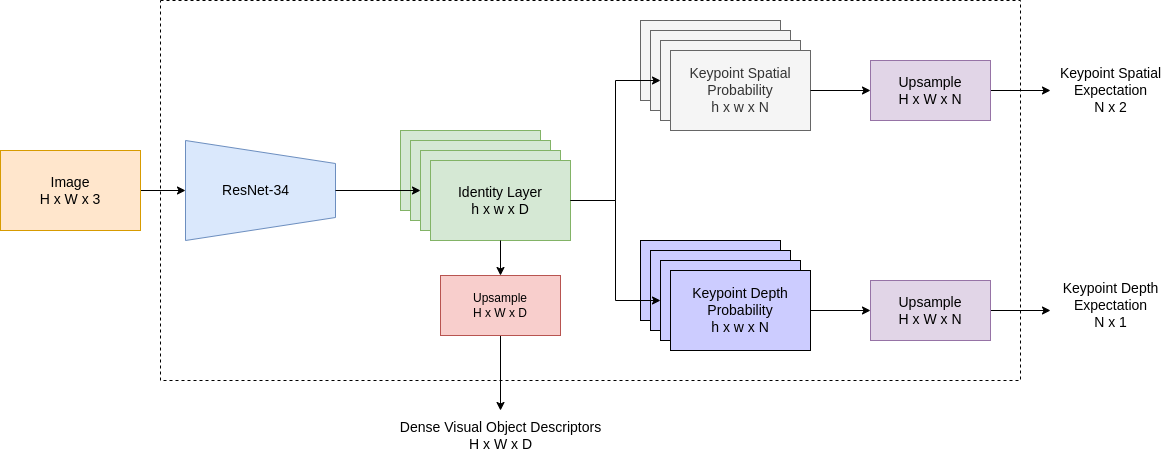
\includegraphics[scale=0.34]{images/arch.png}
    \caption{Illustration of the novel framework designed to compute and seamlessly extract dense visual object descriptors efficiently.
        During inference, we extract dense visual object descriptors directly from the network and ignore predicted spatial-depth expectations of the keypoints.}
    \label{fig:modified_dnn}
\end{figure}


\subsection{Loss Functions}

For training, we directly adopt silhoutte consistency loss ($\mathcal{L}_{obj}$), variance loss ($\mathcal{L}_{var}$) and separation loss ($\mathcal{L}_{sep}$) functions from \cite{suwajanakorn2018discovery} to train the network on the keypoint prediction task.
However, we modify the multi-view consistent loss and relative pose estimation loss. In the case of multi-view consistency loss we
project the predicted spatial-depth expectation using camera intrinsics as follows:
\begin{equation}
    X_{cam} \in \mathbb{R}^{3 \times 1} = \mathcal{I}_{cam}^{-1}  \ [u, v, 1.0]^T \times d \text{ , where  } \ \mathcal{I}_{cam} \in \mathbb{R}^{3 \times 3} \text{ and }  u, v, d \in \mathbb{R}^+.
\end{equation}

Furthermore, we project the camera coordinates of the keypoints from one camera viewpoint to another camera viewpoint using relative transformation supplied from the synthetic augmentation procedure as follows:

\begin{equation}
    \label{eqn:mvc}
    \mathcal{L}_{mvc} \in \mathbb{R} = \mathcal{H}(\hat{X}^B_{cam}, \mathcal{T}_{A \rightarrow B} \hat{X}^A_{cam}) \text{ , where  } \hat{X}_{cam}=[X_{cam}, 1.0]^T \in \mathbb{R}^{4 \times 1} ,
\end{equation}


In Equation~\ref{eqn:mvc}, $ \mathcal{T}_{A \rightarrow B} \in SE(3)$ is a Special Euclidean Group~\cite{thurston2014three} which
is relative transformation from camera-frame $A$ to camera-frame $B$. We use Huber loss $\mathcal{H}$ as it produces smoother gradients for framework optimization.
Furthermore, we do not discard the relative transformation information to calculate the relative pose loss as suggested in \cite{suwajanakorn2018discovery}.
Moreover, being influenced from \cite{zhao2020learning} we modified the relative pose loss as follows:
\begin{equation}
    \mathcal{L}_{pose} = \Vert log(\mathcal{T}_{truth}^{\dagger} \mathcal{T}_{pred}) \Vert \text{ , where  } \ log: SE(3) \rightarrow \mathfrak{se}(3) \text{ and } \mathcal{T}^{\dagger} = \begin{bmatrix}
        R^T & -R^T t \\
        0^T & 1
    \end{bmatrix}.
\end{equation}


\subsection{Robot Grasping Pipeline}
To use the proposed framework as a robot grasping pipeline, we extract dense visual object descriptors from the network and store
one single descriptor of objects in a database manually for now. During inference, we extract dense visual object descriptors from the network and
query the descriptor from the database to find the closest match as follows:
\begin{equation}
    \label{eqn:gaussian_kernel}
    \mathbb{E}{[u^*, v^*]_{d}} = \operatorname*{argmin}_{u, v} \ exp-\left(\dfrac{\|I_D[u, v] - d\|}{exp(t)}\right)^2 \text{ , where  } \|I_D[u, v] - d\| \in \mathbb{R}^{H \times W}.
\end{equation}
Where $t \in \mathbb{R}$ controls the kernel width influencing the search space to compute the optimal spatial expectation $\mathbb{E}{[u^*, v^*]_{d}}$ of
the query descriptor $d \in \mathbb{R}^D$ in the descriptor image $I_D \in \mathbb{R}^{H \times W \times D}$. The computed spatial expectation is projected to the robot frame using camera intrinsics and poses to perform a pinch grasp.
Furthermore, the Franka Emika 7-DOF robot manipulator with two jaw gripper and wrist-mounted Intel Realsense D435 camera is used as a testing setup as illustrated in Figure~\ref{fig:robot_setup}.

\begin{figure}[htb]
    \centering
    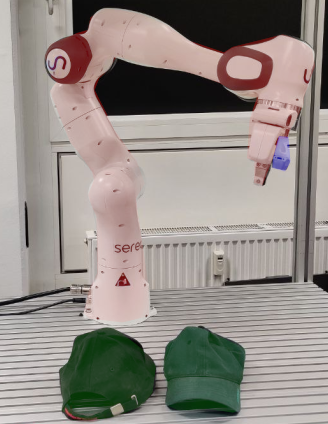
\includegraphics[scale=0.25]{images/franka.png}
    \caption{Illustration of the robot grasping pipeline setup. In the image, the robot is highlighted in red, the caps in green, and the camera in blue.}
    \label{fig:robot_setup}
\end{figure}

\section{Experiments \& Results}
In this section, we outline the benchmarking results employed from the methodologies.
We benchmark the DON framework with Pixelwise NT-Xent loss as in \cite{adrian2022efficient} and our framework with the
proposed loss function with $AUC \pm \sigma$ for $PCK@k, \forall k \in [1, 100]$ metric.
Furthermore, we benchmark the computational resource consumption of the DON framework and our framework.
We also demonstrate the application of our framework as a robot-grasping pipeline in two methodologies,
one of which our framework demonstrates its capabilities to produce object-specific 6D poses for robot grasping.

\subsection{Dense Object Nets}
We implemented training and benchmarking using ``PyTorch-Lightning''\cite{falcon2019pytorch} and ``PyTorch''\cite{paszke2019pytorch} libraries.
Furthermore, we employ
ADAM\cite{kingma2014adam} optimizer to optimize the model for 2500 epochs with a learning rate of
$\alpha = 3 \times 10^{-4}, \beta_1 = 0.9 \text{ and } \beta_2 = 0.999$ with weight decay $\eta =10^{-4}$ to benchmark the DON with Pixelwise NT-Xent loss as in ~\cite{adrian2022efficient}
with a fixed batch size of 1 and 128 image-pair correspondences.
As per the benchmarking results in Table~\ref{table:don_training_results}, the descriptor's robustness increases as the descriptor's dimension gets longer.

\begin{table}[htb]
    \caption{Benchmark of DON framework for GPU consumption and $AUC \pm \sigma$ for $PCK@k,  \forall k \in [1, 100]$ metric.}
    \label{table:don_training_results}
    \centering
    \begin{tabular}{lllll}
        \toprule
        \multicolumn{5}{c}{DON benchmark}                                                                     \\
        \midrule
        Descriptor Size ($D$) & $3 $              & $8 $              & $4 $              & $32$              \\
        AUC for $PCK@k$       & $0.922 \pm 0.006$ & $0.933 \pm 0.011$ & $0.948 \pm 0.012$ & $0.953 \pm 0.008$ \\
        VRAM Usage (GB)       & $9.377 $          & $13.717 $         & $20.479 $         & $30.067$          \\
        \bottomrule
    \end{tabular}
\end{table}

The $AUC \pm \sigma$ for $PCK@k, \forall k \in [1, 100]$ is computed with 256 image-pair correspondences and
the metrics mean and std. deviation is calculated from benchmarking 3 DON models trained for a single descriptor dimension.
We could not train the descriptor dimension of 64 and 128 due to the limited VRAM. Furthermore, to inspect the
results of trained DON, an interface is built using the PyGame library~\cite{pygame} to visualize the results of the trained DON.
The mouse pointer in the image space is mapped to the pixel, and the descriptor at that pixel is queried in another image-descriptor space.
We further use the spatial probability of the descriptor to visualize the queried descriptor
in the image space using Equation~\ref{eqn:gaussian_kernel}
Identify if there are any multi-modal spatial activations in the descriptor spaces and none, as shown in Figure~\ref{fig:check_don}.

\begin{figure}[htb]
    \centering
    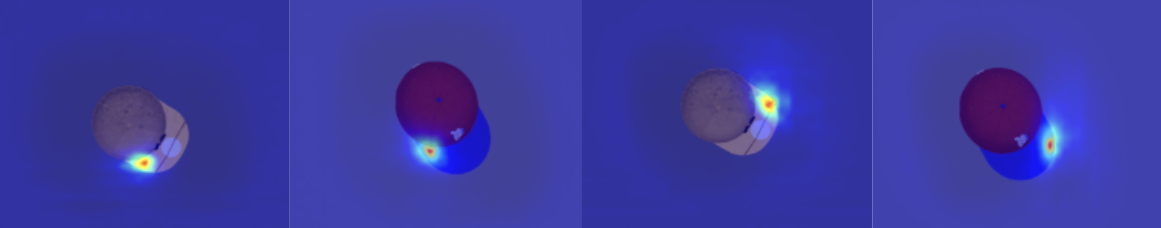
\includegraphics[scale=0.25]{images/test_don.png}
    \caption{Depiction of the spatial probability heatmaps of the descriptor in the image space. We set the temperature in the Equation~\ref{eqn:gaussian_kernel} to $1.1$
        and render the spatial probability heatmaps in the interface. The first and second image from the left and the right highlights the semantically equivalent descriptors in the image space.}
    \label{fig:check_don}
\end{figure}


\subsection{Our Framework}

To train our framework, we employ an ADAM optimizer to optimize the model for 2500 epochs with a learning rate of
$\alpha = 1 \times 10^{-3}, \beta_1 = 0.9 \text{ and } \beta_2 = 0.999$ with no weight decay.
We further use a fixed batch size of 1 and the StepLR scheduler with a step size 2500 and a gamma of 0.9 to train the model with all the loss weights to $1.0$ except variance loss weight to $1 \times 10^{-3}$.
At first, we trained our model with 16 keypoints with a margin of 10 pixels as a hyperparameter for the separation loss, and later, we trained the models with 128 keypoints with a margin of 2 pixels.

\begin{table}[htb]
    \caption{Benchmark of our framework for GPU consumption and $AUC \pm \sigma$ for $PCK@k,  \forall k \in [1, 100]$ metric.}
    \label{table:framework_training_results}
    \centering
    \begin{tabular}{lllll}
        \toprule
        \multicolumn{5}{c}{Our framework with 16 keypoints}                                                          \\
        \midrule
        Descriptor Size ($D$)        & $64 $             & $128 $            & $256 $            & $512$             \\
        $AUC \pm \sigma$ for $PCK@k$ & $0.922 \pm 0.006$ & $0.933 \pm 0.011$ & $0.948 \pm 0.012$ & $0.953 \pm 0.008$ \\
        VRAM Usage (GB)              & $3.799 $          & $4.191 $          & $5.241 $          & $7.341$           \\ \hline
        \multicolumn{5}{c}{Our framework with 128 keypoints}                                                         \\
        \midrule
        Descriptor Size ($D$)        & $64 $             & $128 $            & $256 $            & $512$             \\
        $AUC \pm \sigma$ for $PCK@k$ & $0.922 \pm 0.006$ & $0.933 \pm 0.011$ & $0.948 \pm 0.012$ & $0.953 \pm 0.008$ \\
        VRAM Usage (GB)              & $4.913 $          & $5.409 $          & $6.551$           & $7.915$           \\
        \bottomrule
    \end{tabular}
\end{table}


\subsection{Robot Grasping Pipeline}

For the robot grasping pipeline, we trained our framework with actual caps.
As the synthetic data generation only needs mask and depth information, we could create a mask in no time.
Additionally, while training the framework, we do not need the actual real-world depth information as it computes its own.
We later extracted the dense visual local descriptors from the framework.
We visually inspected for any inconsistencies in the descriptor space, as shown in Figure~\ref{fig:check_real_caps},
and found it consistent. Furthermore, we did not use the models trained on the synthetic dataset, as the representations were inconsistent with the real caps.

\begin{figure}[htb]
    \centering
    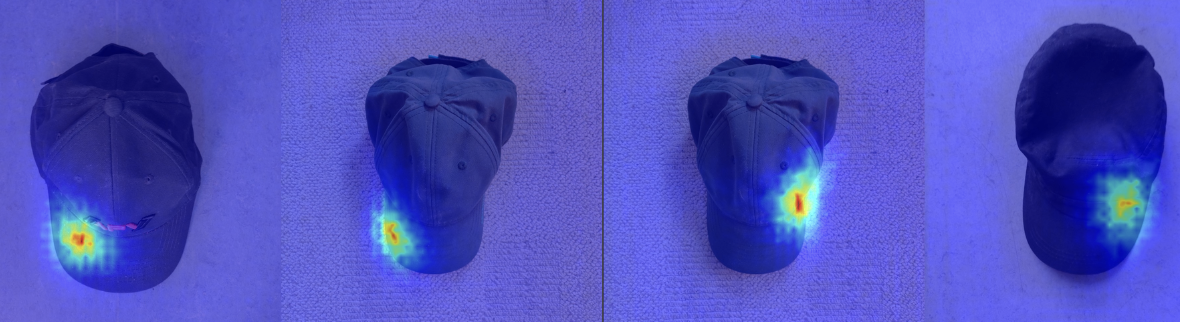
\includegraphics[scale=0.15]{images/test_real_caps.png}
    \caption{Visual inspection of the dense visual descriptors space of the real caps.}
    \label{fig:check_real_caps}
\end{figure}

For robot grasping, a descriptor is picked from the descriptor space and queried in real-time such that robot can pinch-grasp the object.
We could successfully grasp the caps with the robot, as shown in Figure~\ref{fig:straight_grasp}.

\begin{figure}[htb]
    \centering
    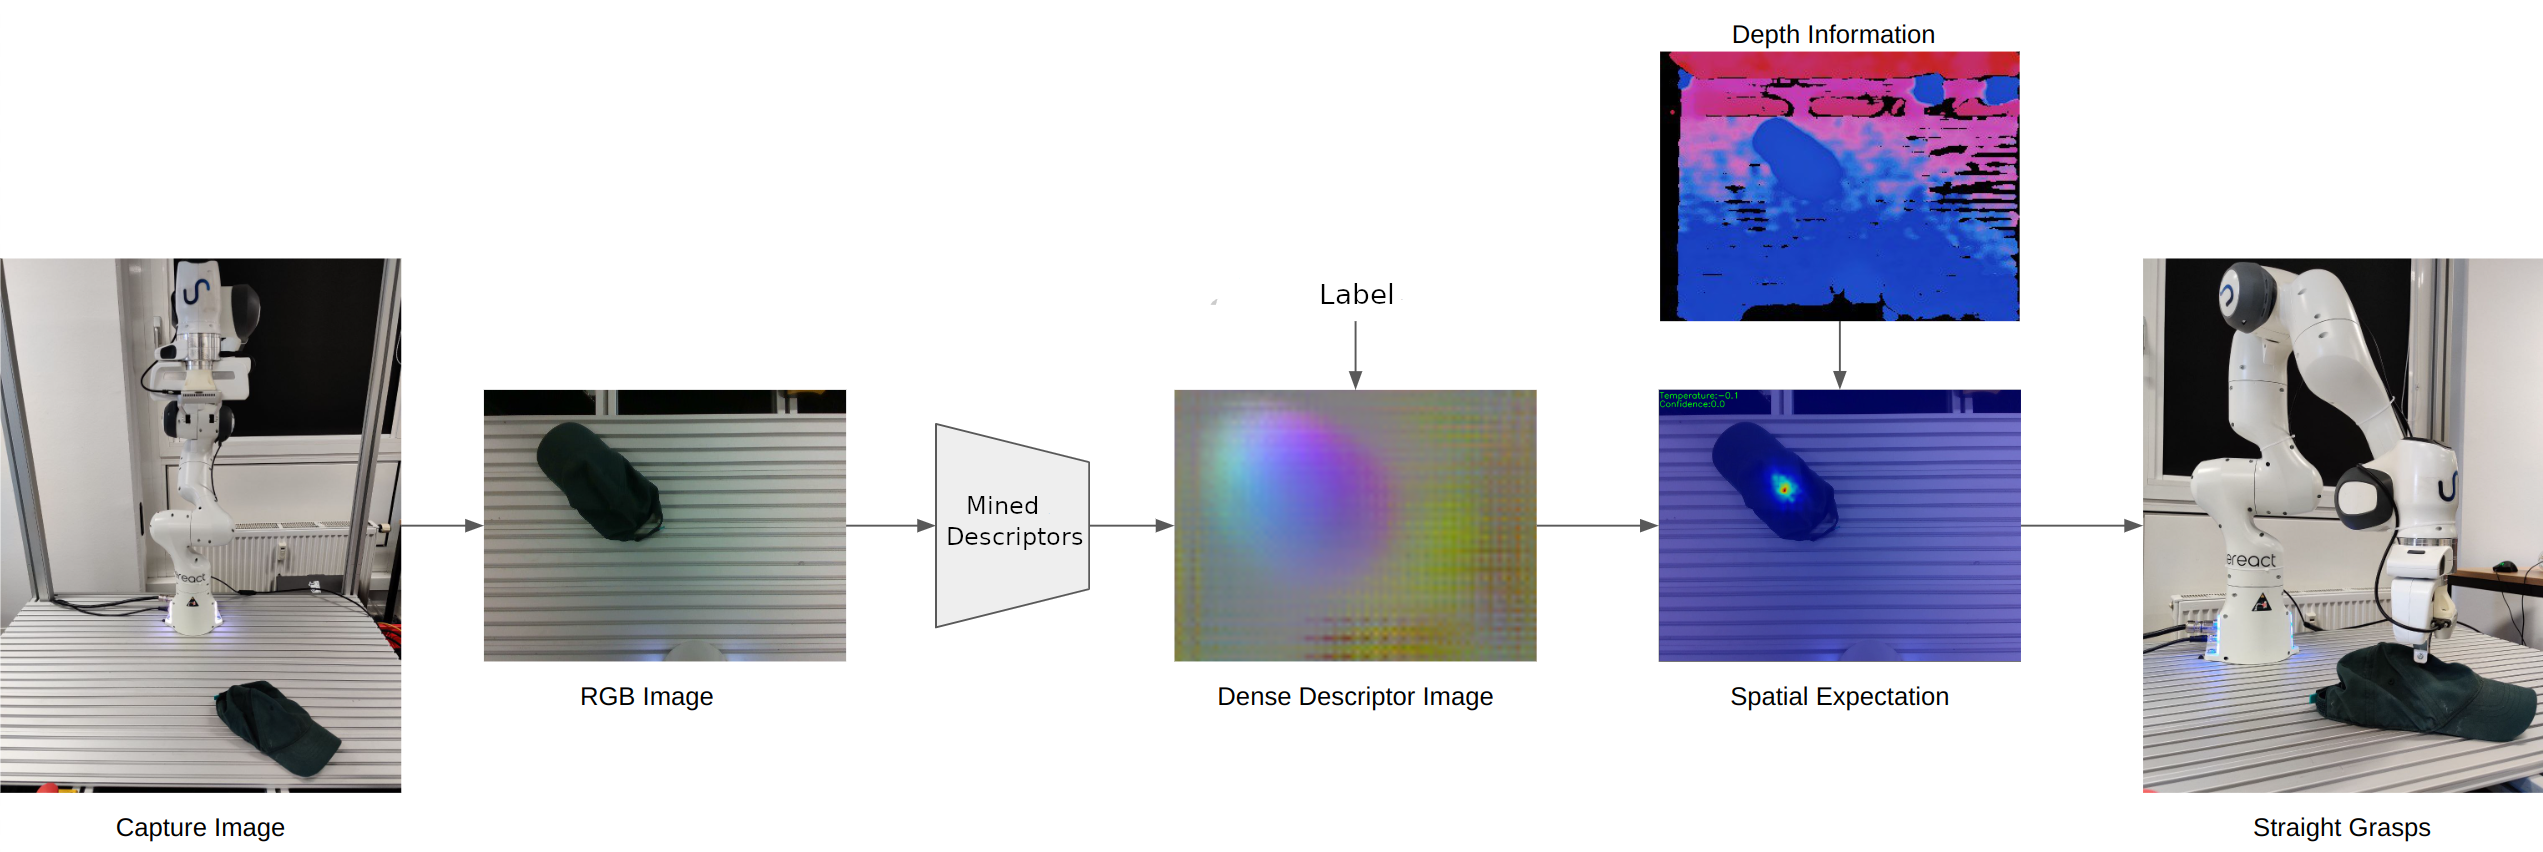
\includegraphics[scale=0.15]{images/straight_grasps.png}
    \caption{Depiction of the straight robot grasping pipeline.}
    \label{fig:straight_grasp}
\end{figure}

As our framework inertly regresses keypoints on the object, we could use it as an alternative approach to grasp the caps by computing the pose
generated by the keypoints considering the actual depth information instead of network-regressed depth information.
We extract the spatial probability of each keypoint from the framework and deactivate spatial probabilities where the depth information is missing,
as the depth image from the camera is noisy. Furthermore, the spatial expectations of the keypoints are projected to the camera frame
to calculate a 6D pose in the camera frame. The 6D pose is transformed in the robot frame to perform an aligned grasp, as shown in Figure~\ref{fig:aligned_grasp}.

\begin{figure}[htb]
    \centering
    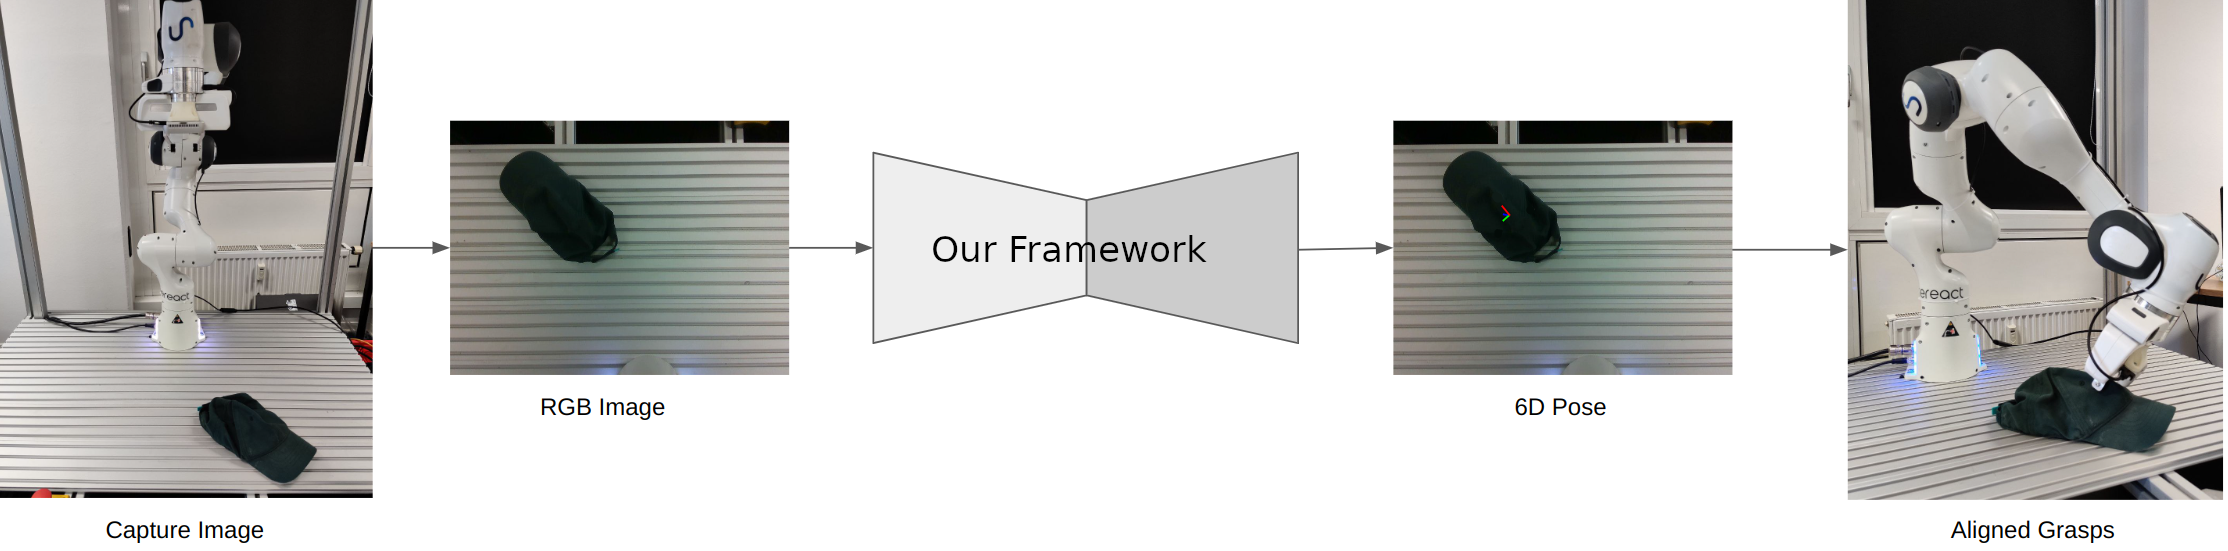
\includegraphics[scale=0.17]{images/aligned.png}
    \caption{Illustration of the aligned robot grasping pipeline.}
    \label{fig:aligned_grasp}
\end{figure}

\section{Conclusion}
This paper introduces a novel framework for mining dense visual object descriptors without explicitly training DON. We have successfully
eliminated the requirement for image-pair correspondence mapping in training DON by employing synthetic augmentation data generation and a novel deep-learning architecture.
Our benchmarking results showcase the effectiveness of our framework in generating robust and denser visual local descriptors.
However, it needs to outperform the original DON framework in robustness.
Moreover, a notable advantage of our proposed framework is its significantly reduced computational resource consumption,
amounting to a remarkable 86.67\% decrease compared to the originally proposed framework.
It is important to note that our current framework is limited to single object-dense visual descriptors. Nevertheless,
we have plans to extend our methodology to encompass the production of multi-object dense visual descriptors in cluttered scenes.
By doing so, we aim to enhance the versatility and applicability of our framework in real-world scenarios.
To demonstrate the practicality of our framework, we have integrated it into a robot-grasping pipeline using two distinct methodologies.
Remarkably, our framework can generate object-specific 6D poses, enhancing robot grasping performance.
This successful application further highlights the potential utility of our framework in real-world robotic systems.

\printbibliography

\end{document}
